\section{Introduction}~\label{sec:intro}

%% dbms adopting to SSD characteristics
\module{Modern DBMSs optimize for SSD characteristics.}
\revision[R3.W1]{
As SSD prices have continued to fall while DRAM costs stagnate, SSDs have replaced disks as the primary storage medium for high-performance DBMSs~\cite{DBLP:journals/pvldb/Leis24, scalestore, CFLRU, flashalloc, DBLP:conf/fast/ManeasMES22}.
Consequently, modern systems increasingly tailor their designs to SSD properties, 
such as internal parallelism~\cite{DBLP:journals/pvldb/HaasL23}, read-write asymmetry~\cite{DBLP:journals/pvldb/LeeAL23, WAR, DBLP:journals/pvldb/VohringerL23}, and SSD reads~\cite{readpriority, hidinglatency}.}

%%% SSDs are used in database systems but still do not account for writes.
\module{Yet most DBMSs still do not optimize for SSD writes.}
However, few systems control database \emph{write behavior} to optimize for SSDs, even though SSDs handle writes very differently from hard disks. 
The overall SSD performance for out-of-memory workloads can be greatly impacted by how a database system writes to the device.
Furthermore, SSDs have a finite lifespan: each write wears out flash cells, unlike hard disks, which do not suffer from endurance limits~\cite{lerner2024principles, SSDhistory}.
However, despite these differences, most systems still issue writes as if targeting hard disks -- ultimately writing far more than intended while remaining unaware of the consequences.

\begin{figure}[t]
      \setlength{\abovecaptionskip}{3pt} % space above caption
  \setlength{\belowcaptionskip}{0pt} % space below caption (usually inside float)
    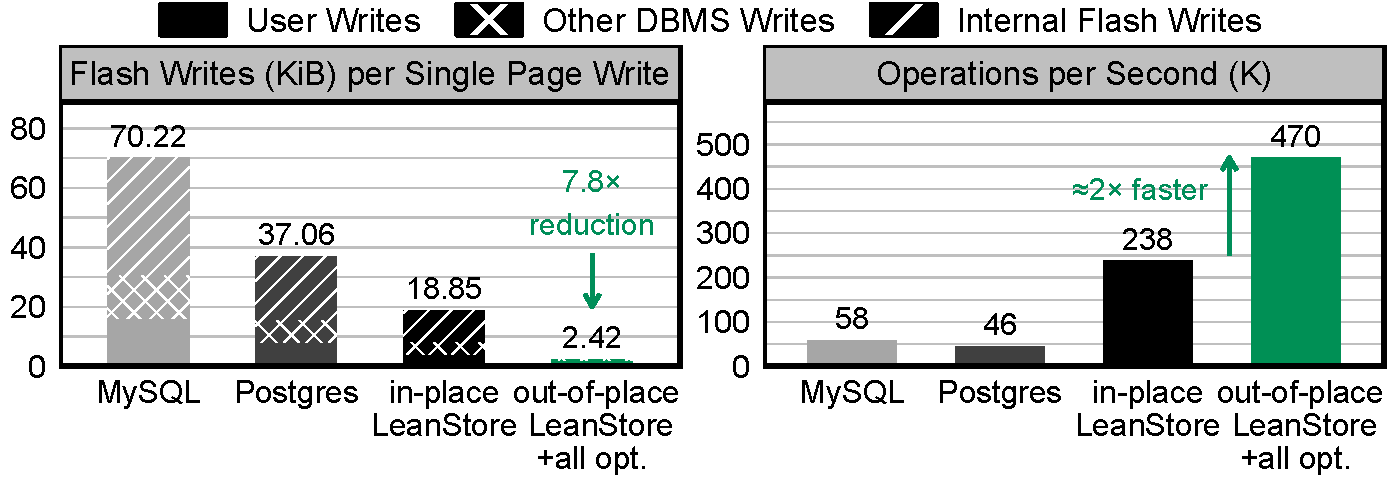
\includegraphics[clip, width=\columnwidth]{figures/intro.pdf}
    \caption{Flash writes per single page write and throughput (YCSB-A zipf $\theta$ = 0.8, Samsung PM9A3 SSD 90\% full, page sizes (KB): MySQL: 16, PostgreSQL: 8, LeanStore: 4)} 
    \label{fig:intro} 
    \vspace{-3mm} 
\end{figure}

\module{Database systems write significantly more than expected.}
Once database writes accumulate beyond a certain threshold, ignoring SSD write characteristics becomes increasingly costly~\cite{ssdiq}.
We benchmark the B-tree-based engine LeanStore~\cite{DBLP:journals/pvldb/Leis24} on an enterprise SSD filled to 90\% using the YCSB-A workload (zipf $\theta$ = 0.8), 
running it until cumulative DB writes exceed four times the SSD’s capacity.
Surprisingly, as shown in the third bar of the first plot in \cref{fig:intro}, the in-place-write LeanStore baseline writes 18.85 KiB per 4 KiB B-tree node page write, 4.7$\times$ more than expected.
A similar trend appears in MySQL and PostgreSQL, as shown in the first two bars.

\module{Identifying the cause of write amplification.}
To investigate the source of the amplification, we categorize writes into three types (ignoring WAL writes because they are easy to handle):
(1) user writes (including evictions or checkpointing),
(2) additional DBMS-issued writes, and
(3) SSD-internal writes (obtained by OCP~\cite{ocp}). 
%(obtained by Open Compute Project (OCP) command).
Here, we identify two main culprits behind this amplification.

%% and also show that doing out-of-place writes with LSM tree doesn't solve anything
\module{Culprit 1: DBMSs themselves write more.}
The DBMS often issues more writes than expected.
When comparing the user writes with the total amount of writes issued by the DBMS (user + other DB-issued writes) in \cref{fig:intro}, 
it is roughly \emph{double} the user writes due to the doublewrite buffering overhead.
This behavior is typical of in-place systems, including MySQL~\cite{mysql-dwb} and PostgreSQL (albeit indirectly)~\cite{postgresql/doc/dwb}, as shown in the first two bars in \cref{fig:intro}.

\module{Culprit 2: SSDs internally amplify DBMS writes.}
The SSD itself amplifies DBMS writes, a phenomenon known as SSD \emph{write amplification} (WA).
In our experiment, LeanStore experiences a Write Amplification Factor (WAF) of 2.36$\times$ (\cref{fig:intro}), meaning total flash writes are 2.36$\times$ the DBMS-issued writes.
%\revision[R2.D8]{We also find similar or even higher amplification when using filesystems such as ext4 (2.41), F2FS (2.48), or XFS (2.14) in a separate experiment.}
This internal WA degrades performance over time and reduces SSD lifespan~\cite{lerner2024principles, arkiv/Dayan15}.
The Samsung PM9A3 data center SSD used in the experiment guarantees a lifetime of 5 years at 1 Drive Write Per Day (DWPD)---corresponding to an average write speed of only 11~MB/s.
LeanStore writes about 400~MB/s in the experiment, which means that the SSD would reach its endurance limit in about 1.5 months.

%% the case for total WAF
%% SSD filesystem cannot solve it
%% Out-of-place write befcomes necessary
\revision[R2.D1]{
\module{DBMS taking charge of minimizing end-to-end WA.}
A single page write is amplified first within the DBMS and then within the SSD, yielding a total WAF of DB~WAF~$\times$~SSD~WAF.
Conventionally, minimizing SSD WAF is delegated to lower layers---either the SSD or, indirectly, the filesystem~\cite{DBLP:conf/usenix/BjorlingAHRMGA21,DBLP:conf/fast/LeeSHC15,DBLP:journals/pvldb/KangCOL20}, 
while DB WAF is treated separately (e.g., LSM-tree WA optimizations~\cite{DBLP:journals/tos/LuPGAA17,rocksdb-saf}).
However, DBMS write issuance dictates both DB and SSD behavior; 
focusing only on DB WAF can paradoxically increase flash writes when SSD WAF is overlooked.
Thus, we argue that the DBMS, with the most workload knowledge at the highest layer, should coordinate writes with both DB- and SSD-level WA in mind.

\module{Reducing SSD writes with out-of-place techniques.}
To minimize flash writes per operation, we first move from in-place to out-of-place updates.
By removing the constraint of rewriting a page at a fixed location, the DBMS gains \emph{flexibility} in write placement. 
We then present several out-of-place-based optimizations that together minimize end-to-end WAF. }
These are implemented on LeanStore after converting to out-of-place writes. 
Using the same benchmark, the results (shown in the final bar of the two plots in \cref{fig:intro}) 
demonstrate that our out-of-place design with optimizations reduces flash writes by \emph{7.8$\times$} per operation compared to in-place LeanStore. 
This reduction is achieved by eliminating all other redundant writes, effectively reaching the near-optimal level of user writes alone.
Consequently, SSD lifespan is directly extended, while cost, power consumption, and carbon footprint per operation are reduced~\cite{carbon,DBLP:journals/usenix-login/Arpaci-Dusseau17}.
Throughput (operations per second, OPS) nearly doubles as well (right panel of \cref{fig:intro}).

\module{Contributions.}
\revision[R2.W1]{
The proposed optimizations systematically reduce cross-layer WA 
by considering how the write pattern shapes DB- and SSD-level amplification and their interplay.
Our design requires only modest changes to upper components of the storage engine, including the buffer pool, logging/recovery, and index structure, making it readily applicable to other B-tree-based systems.
The proposed optimizations are:}

\vspace{-1mm}  % reduces vertical space below the figure
\begin{itemize}[left=0.2cm]
\item \textbf{Compression \& page packing}:
\revision[R2.D4]{  
Page-wise compression reduces write volume, but with 4~KiB pages, its benefits vanish when compressed pages are misaligned or smaller than 4~KiB.
We introduce page packing, grouping compressed pages so each is read with a single 4~KiB access while retaining write and space savings.}

\item \textbf{Grouping by deathtime}:  %  (\cref{sec:GDT})
System-level out-of-place writes inherently require garbage collection (GC).  
To minimize WA during GC, we group pages by their expected invalidation time (``deathtime'') when placing them, derived from DB semantics.  

\item \textbf{ZNS support}:  %  (\cref{sec:zns})
Our design naturally extends to Zoned Namespace (ZNS) SSDs, leveraging the existing DB GC and mapping.  
This enables full compatibility with ZNS, which inherently guarantees an (optimal) SSD WAF of 1.  

\item \textbf{Aligning DB and SSD GC units}:  %  (\cref{sec:fdp})
For non-ZNS SSDs, SSD GC-induced WA is mostly inevitable.
By estimating the physical placement inside SSDs, 
we find that the first key to mitigate SSD WAF is to align the DB GC unit with the SSD’s internal GC unit.  
When available, this is achieved using the FDP Reclaim Unit size; 
otherwise, it can be estimated using a ZNS-like pattern.

\item \textbf{NoWA pattern}:  %  (\cref{sec:nowa})
For commodity non-ZNS SSDs not featuring FDP, we introduce a NoWA (No Write Amplification) pattern that guarantees SSD WAF $~=$ 1, 
even at full device utilization.  
\revision[]{
\item \textbf{Using FDP placement hints}:  
For FDP-enabled SSDs, we show how to use placement hints that can replace the NoWA pattern.}
\vspace{-1mm} 
\end{itemize}
\noindent
\revision[R2.W1]{
The first two DB WAF optimizations are orthogonal yet complementary, 
while the remaining SSD-side optimizations may be chosen based on the underlying device.
Importantly, applying only the DB WAF optimizations without the SSD WAF ones can increase total WAF; 
the full set should therefore be viewed jointly.
In \cref{sec:oop}, we first motivate why the DBMS is best positioned to optimize SSD writes and why this necessitates out-of-place updates. 
We then present each optimization as structured in the figure below:
}
\begin{center}
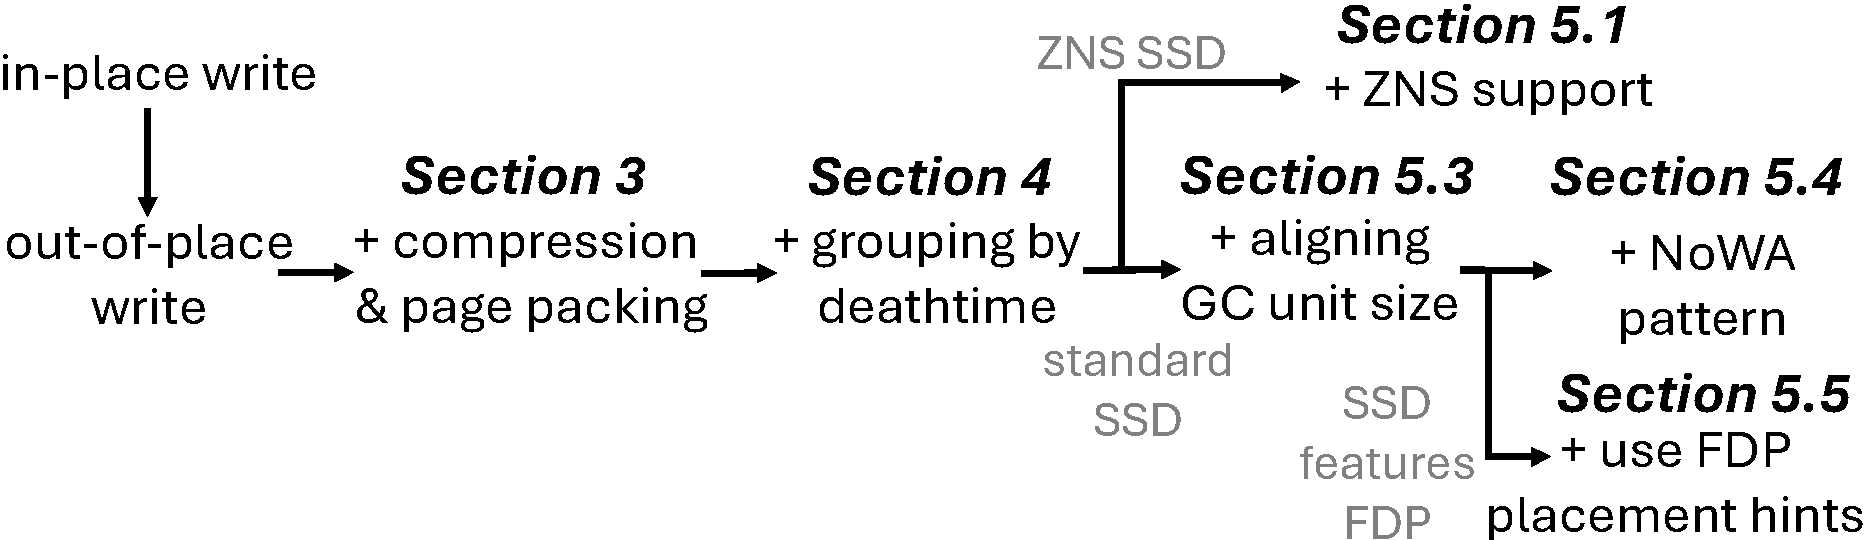
\includegraphics[clip, width=0.95\columnwidth]{figures/roadmap.pdf}
\end{center}
%\vspace{-3mm}  % reduces vertical space below the figure
